\chapter{Simulations}
To study the effect compensatory mutation have on Muller's ratchet, the discrete system described in
Section~4.1 was implemented in Java\footnote{\url{http://www.java.com}} using the Colt libraries for
High Performance Scientific Computing\footnote{\url{http://acs.lbl.gov/software/colt}} developed by the
European Organization for Nuclear Research (CERN). The software is named
\emph{mrj} (for Muller's ratchet in Java) and is freely available precompiled
and in source code at the authors
homepage\footnote{\url{http://paulstaab.de/science}}. The source code can also
be found in Appendix \ref{ap:source_code}.

By default, the software starts with a population free of mutations. To
simulate the reproduction according to Muller's ratchet with compensatory mutations, two alternative
methods were implemented. As default, the function \emph{reproduction\_normal()} is used, which is a
straight forward implementation of the discrete dynamics. For each of the $N$ individuals, there is
first sampled a parent according to the multinomial distribution with parameters according to the
fitness and distribution of the types in the generation before. Then there is a
binomial distributed number of mutations removed and a Poisson distributed
number added again afterwards. Finally the type frequencies are calculated. The
alternative reproduction function \emph{reproduce\_alternative()}, which can be
activated via the command line option '-a', first calculates the expected type
frequencies $p_k$ as in \eqref{cm:eq:p_k-def} for a reasonable number of types
$k$ including mutations and compensatory mutations, and does a multinomial sampling
of $N$ individuals according to the expected frequencies afterwards.

However, as we could not measure a
significant difference in run time of both methods (Figure \ref{sim:f:runtimes}), we stuck to the
default for our simulations. Note that the run times kept roughly constant even for
moderate large values of $N$.

\begin{figure}[h]
\centering
\begin{tabular}{ccc} 
%\toprule %
$N$ 	& normal 	& alternative \\
$10^2$ 	& 4:52 		& 4:55\\
$10^3$ 	& 4:48 		& 4:55\\
$10^4$ 	& 4:50 		& 4:49\\
$10^5$ 	& 28:53 	& 29:48
\end{tabular}
\caption{Run times of a simulation of $10^5$ generations using \emph{reproduction\_normal()}
respectively \emph{reproduce\_alternative()} for populations of different size $N$ with $\lambda =
0.1$, $\alpha = 0.03$ and $\gamma = 10^{-4}$.}
\label{sim:f:runtimes}
\end{figure}

\noindent
The simulations itself were carried out for a wide range of parameters on a
distributed grid of twelve desktop computers, better known as the students
'PC-Pool' of the Mathematical Institute in Freiburg. The resulting 1.8 GB of
data were analysed using R (\cite{team_r:_2008}).

First, we examined whether compensatory mutations indeed stop the ratchet. As
expected, that was sooner or later the case for all simulated combinations of
parameters. A typical run consists of a starting phase, where deleterious
mutations are accumulated quickly until a plateau is reached, where the ratchet
attempts to stay but is disturbed by random fluctuation. This is illustrated in
Figure \ref{sim:f:path1}, where the observed mean number of mutations
$\kappa_1(t)$ is drawn for a single run as well as its average.

\begin{figure}[h]
  \begin{center}
	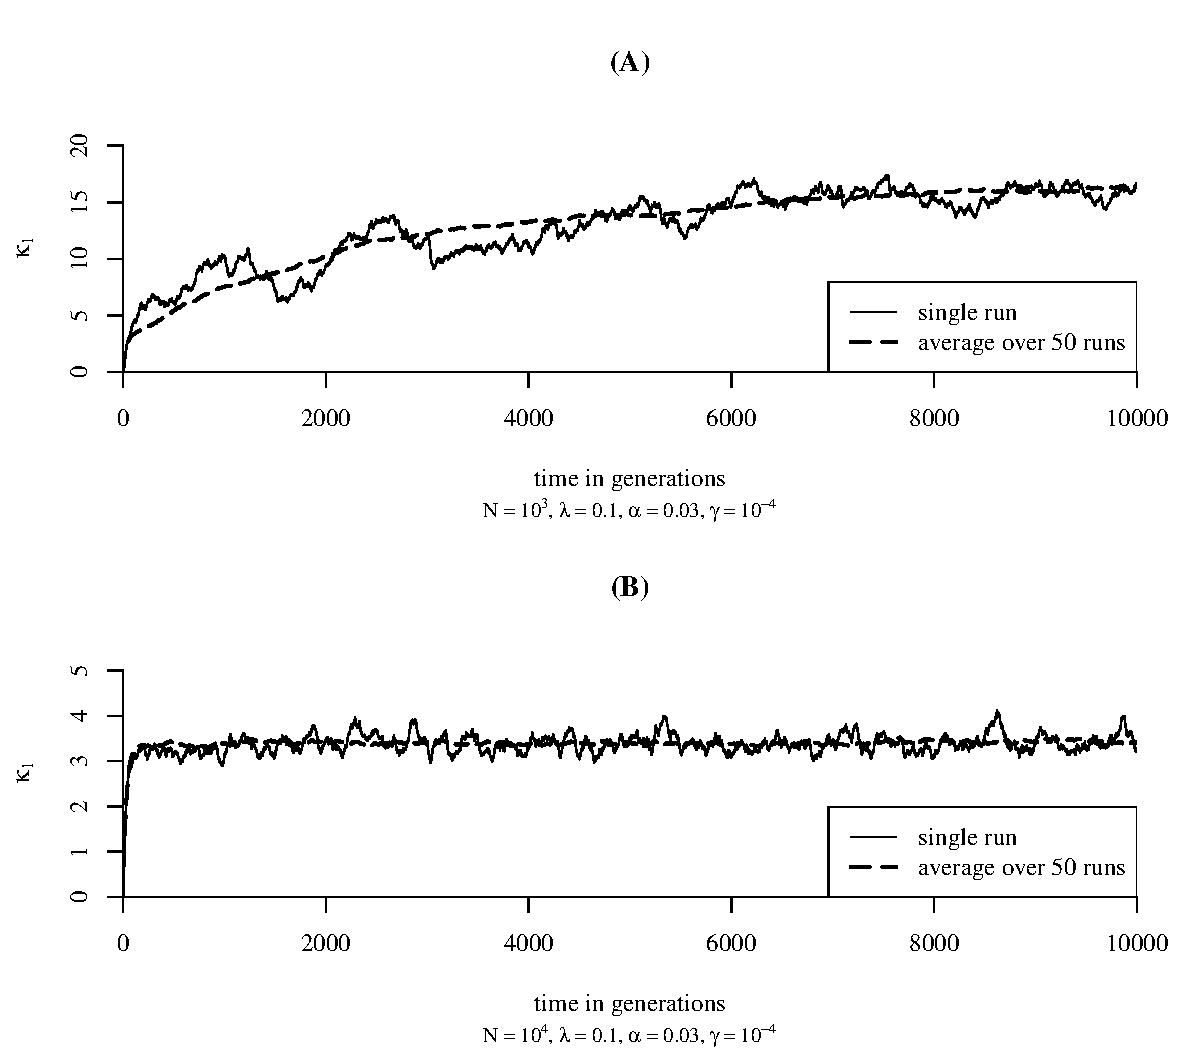
\includegraphics[width=13cm]{img/paths.pdf}
   \end{center}
  \caption{\label{sim:f:path1} The evolution of the average number of
    deleterious mutations $\kappa_1$ is plotted against time. In addition, the
    average over 50 different simulations is drawn.}
\end{figure}

\noindent
The fluctuations are larger for parameters were the ratchet without compensatory
mutation clicks frequently. That is in particular true for small populations as
in Figure~\ref{sim:f:path1}.A. Observe that the plateau lays higher in this
Figure, whereas it almost exactly takes the expectation value $\theta = \lambda / (\alpha +
\gamma)$ of the equilibrium Poisson distribution predicted for $N=\infty$ in
Figure~\ref{sim:f:path1}.B. 

\begin{figure}[h]
  \begin{center}
	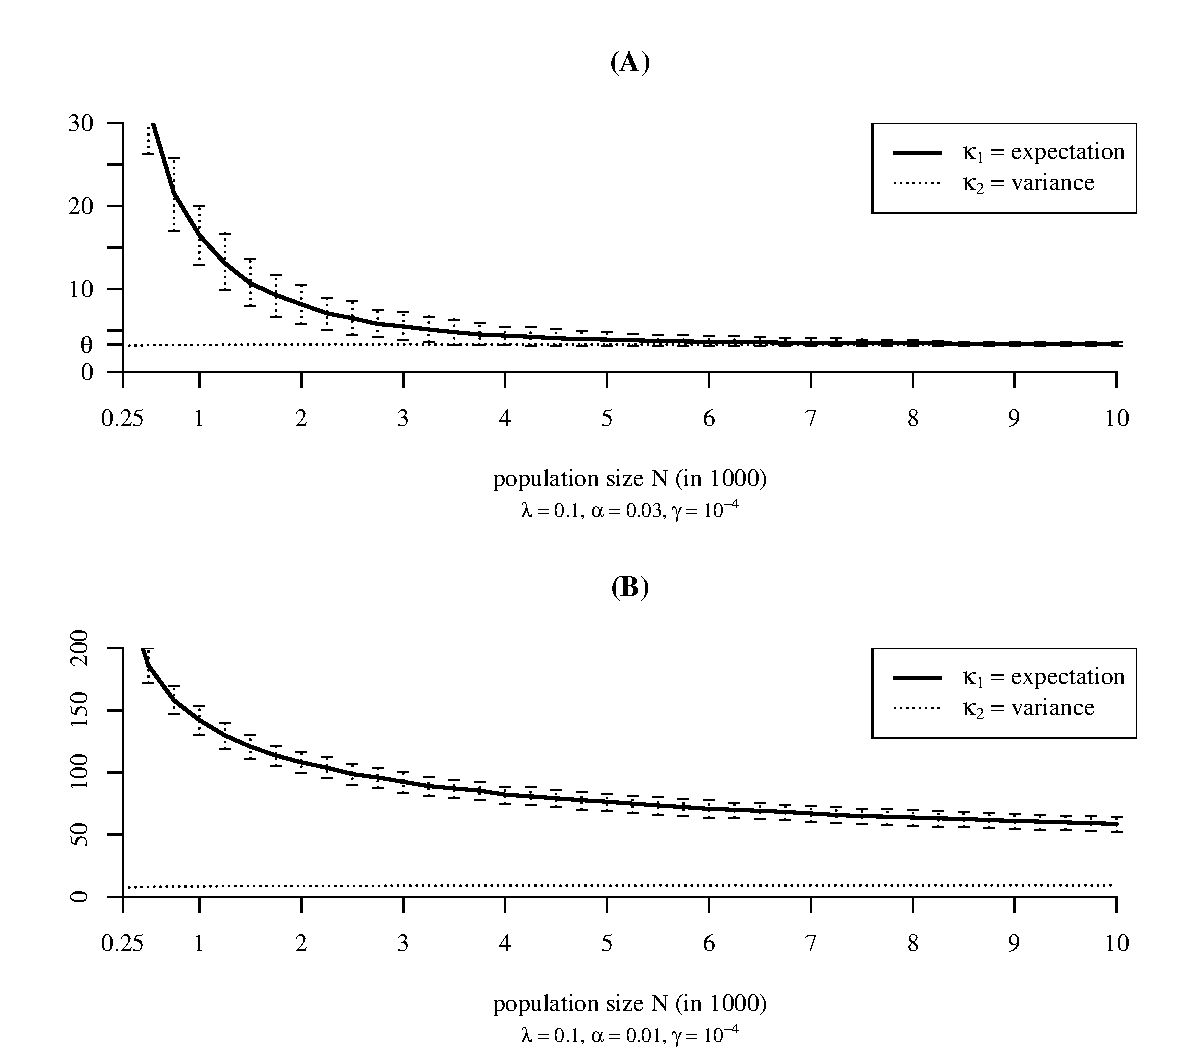
\includegraphics[width=13cm]{img/conv.pdf}
   \end{center}
  \caption{\label{sim:f:konv} The empirical distribution of $\kappa_1$ and
    $\kappa_2$ are evaluated between time $5\cdot 10^2 N$ and $10^3
    N$. The plot for $\kappa_1$ includes the resulting 10\% and 90\%
    quantiles.}
\end{figure}

\noindent
Figure~\ref{sim:f:konv} demonstrates that the magnitude of the ``finite
population effect'' for the ratchet with compensatory mutations is closely
related to the click rate of the classical ratchet. Here, the average value of
$\kappa_1$ \emph{after the ratchet has reached the described plateau} is draw as
function of the population size $N$. In Figure~\ref{sim:f:konv}.A, the
observed value of $\kappa_1$ quickly approaches the prediction $\theta$. Hence,
we can assume that the population is well approximated by the large population
limit even for moderate $N$. Note that the parameters $\lambda = 0.1$,
$\alpha = 0.03$ and $N=10^4$ would lead to approximately 0.34 clicks per $N$
time units without compensatory mutations. To quantify the magnitude of the
fluctuations around the expected value, the 10\%- and 90\%-quantiles of the
empirical distribution of $\kappa_1$ are included as well.

In Figure~\ref{sim:f:konv}.B, $\kappa_1$ is much greater than the
predicted value, even for large populations. As $\alpha = 0.01$ is much smaller here, we would expect
approximately 152 clicks per $N$ time units for $\gamma = 0$ (and again for
$N=10^4$). Hence, we can conclude that our approximations hold if the population size $N$ is sufficiently
large and $\lambda$ and $\alpha$ would not lead to frequent clicks of the normal
ratchet.

\begin{figure}[h]
  \begin{center}
	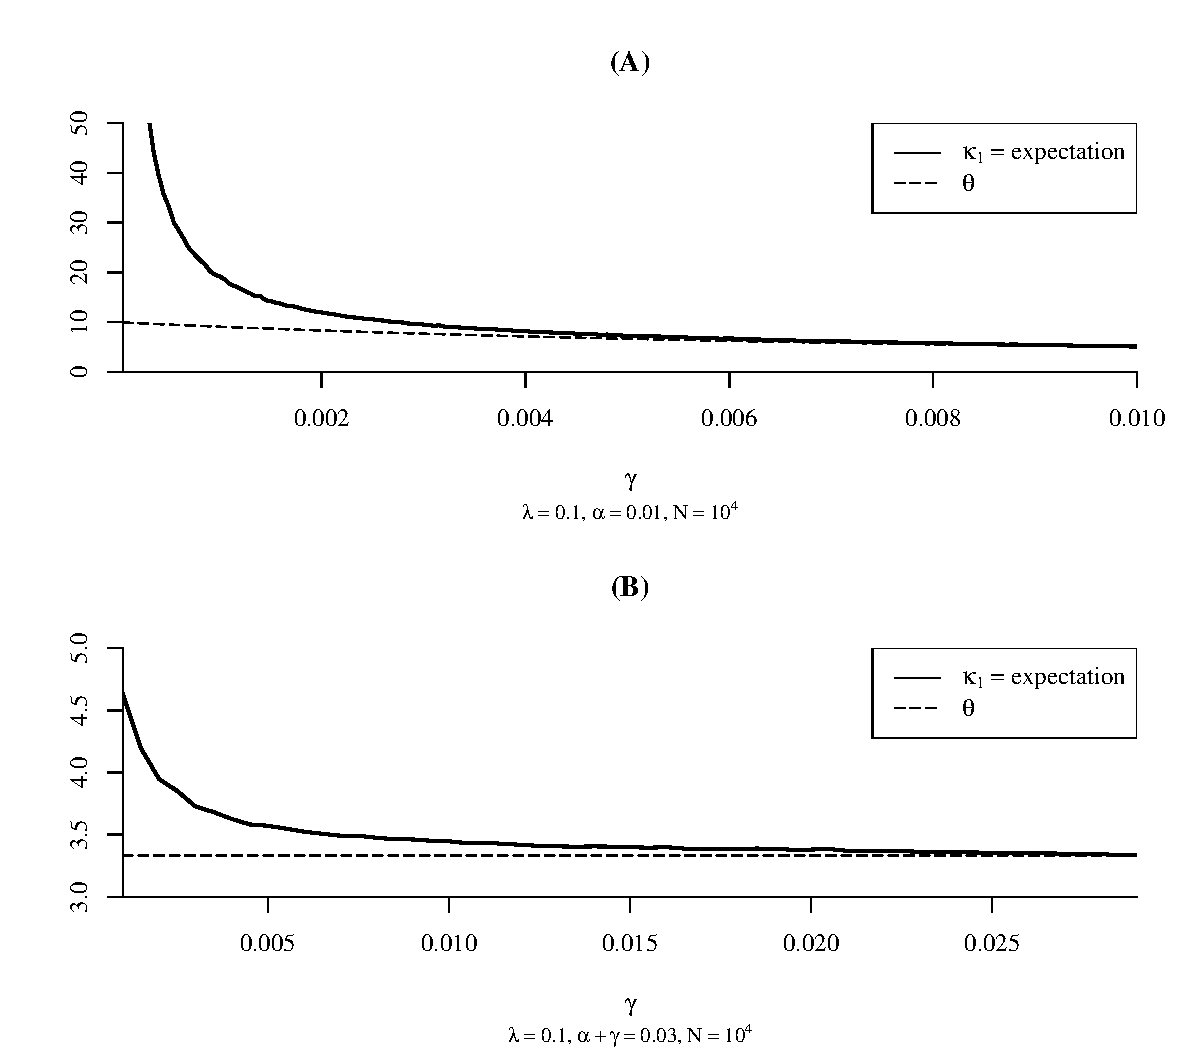
\includegraphics[width=13cm]{img/gammaVSalpha.pdf}
  \end{center}
  \caption{\label{sim:f:dif_gamma} Again average values of $\kappa_1$ are drawn, here for different
  values of $\gamma$. In Figure~(A) $N$, $\alpha$ and $\lambda$ are fixed, whereas $\alpha$ is
  variable in Figure~(B), so that $\alpha + \gamma$ is constant.}
\end{figure}

\noindent
Remarkably, the empirical variance $\kappa_2$ is always close to the variance
of the predicted $\Poi{\theta}$-distribution for all $N$ in both pictures of
Figure~\ref{sim:f:konv}. That suggests that the ratchet with compensatory
mutations is close to a shifted Poisson distribution most of the time.

As illustrated in Figure~\ref{sim:f:dif_gamma}.A, only unrealistic high values
of $\gamma$ assure that frequent clicks become compensated. Note that the
parameters $\lambda$ and $\alpha$ are the same as used in
Figure~\ref{sim:f:konv}.B here. Even though the quality of the approximation
certainly depends on $\gamma$ as well, the click rate of the classical ratchet
seems to be the more important parameter.

Finally we checked, if the symmetry of $\alpha$ and $\gamma$ in $\theta$ is also
reflected for finite population size. However, Figure~\ref{sim:f:dif_gamma}.B
suggests that the purifying effect of compensatory mutations is more important
than the one of selection. This seems reasonable as every mutation can be lost
by a compensatory mutation, while only those ones that an individual has
additional to the least number of mutations in the population can be lost by selection.